\section{Programs, methods and theory use for development}
\phantomsection

\subsection{Problem Definition}

Nowadays social media become an important marketing tool. Beside a big network where everyone can share information and express their thoughts, social media channels represent a good place for advertising different types of products and services. Moreover, people started using social media as a source of helping each others by publishing different advices about how to dress up, how to apply make up and what type of products are good. That is why video blogs that are posting on Youtube are very popular. According to Research Now, 84 \% of people have purchased products based on their descriptions in blogs.\cite{cyber} The percentage is very high, therefore companies are very interested in influential bloggers who can advise their products. 

The problem acquires when stakeholders start researching the influential bloggers. Since the number of Youtube users is huge and it is in permanent growth the researching task is supposed to take a long time and not always to give desired results. Finduber is meant to resolve this problem using a search engine based on lexical analysis process. 

\subsection{Market Analysis}

In order to create a good software it is necessary to make a market research and find similar solutions to the problems that are being solved by those software. Analysing the existing solutions will help to create a tool atractive for companies to use. The bloggers become popular in the last years, that is the reason why there are not so many tools for reaching out to influencers.

On of the existing solutions is self-service tool FameBit that allows brands to outline their expectations for campaigns and receive proposals directly from YouTubers. FameBit’s limitation is that there is no way to filter talent from one long list of proposals to easily find the channel with the best focus and momentum for your brand. They also have brands sign a six-month exclusivity agreement, restricting a company from entering into any deal with the Influencer to create promotional media content.

OpenSlate is another tool that analyzes YouTube API, social media, and media campaigns’ performance data to measure a channel’s performance. As of today, OpenSlate stores data on more than 220,000 channels. However one drawback is that they do not allow you to export data outside of the platform. To use the system it is need to request a request after that to fill in a long form specifying the qulity measures, brand safety, content and others. 

Tubular is similar to OpenSlate. However they differ in the following ways: they operate with data from more than 2 million YouTube Influencers; allow data to be exported; provide a channel’s contact details and network affiliation; and provide additional info about channel’s other social media engagement. The main drawback of the tool is that its search engine is based on influencer's title. Another issue is that it gives a list of top Youtube channels in general, not only bloggers.

To create a list of things that the solution should have, a strong market analysis should be done and a poll through existing companies should be made and as an result of these, the following 4 criteria occured to be the most important in order to solve the problem of time-waste and it to be atractive to the companies to buy as a software:

There are others tools in beta version with similar drawbacks. Bellow is a list of main issues of existing solutions.

\begin{itemize}
\item \textbf{Price:} Most of the existing tools offer only a demo version. In order to use the system functionalities a monthly payment is required. The amount can reach up to 300 \$, depending on selected package.
\item \textbf{Lot of information:} Existing platforms have a very complex user interface. Usually it combines a set of social media channels and mixt them together in the same view. Thus, it becomes complicate to find the suitable influencer for your company through all the data.
\item \textbf{Lack of Simplicity}. All current existing tools require a number of steps in order to find an influencer. They usually offer some other additional services as well and all that brought together makes the service be not that straight forward. In this way for some marketers it takes a while to get used to certain technology.
\end{itemize}

\subsection{Project Specification}

Finduber is a tool used to help stakeholders in finding influential bloggers according to their needs and requirements. Compared to other platforms that provide a general search mechanism among social media users, Finduber is focused on well defined search parameters. More differences and benefits of Finduber project are pointed out in the futher analysed example. 

Let's suppose that a company needs to promote its new product -- a special kind of \textit{soap}. Basically, this means that the search should be performed based on keyword \textit{soap.} An existing tool will return a list of Youtube users that have in their username the keyword that is far not the desired result. Finduber project assign first the keyword to an existing category and after that processes to searching. In this way, the user has the result that he expects.

The core of the search engine is based on machine learning techniques such as lexical analysis, cluster analysis and natural language processing.

In order to make the project real the following plan should be executed:

\begin{enumerate}

\item[--] To create a taxonomy database. 

\item[--] To optimize database with youtube users by grouping it into pre-defined categories .

\item[--] To design a simple web application that will show the research results. 

\end{enumerate}

\textbf{Taxonomy database} aims to hold a category tree for a pre-defined set of industries. For Finduber project are chosen five industries that are more trendy among bloggers and users: Beauty, Fashion, Sports, Games, Food. 

The purpose of creating this database is to assign a given word to an existing category during searching engine process. A detailed explication about methods and technologies used to create the taxonomy database is given in Chapter 3. 

\textbf{Youtube database optimization} is a crucial step of the Finduber project. It represents the second step of the search engine algorithm, given that the engine determined the category to which the inputted by user word belongs. The problem now is how to use the word category for further search. How it can be used to extract required information from the database with youtube users? Obviously, Youtube page does not have the defined categories that Finduber project uses. The solution is to group youtube users from database to categories defined in the application based on their description, username and keywords. Lexical analysis and natural language processing techniques are used to optimize the database. A deeper analyses of these techniques is described further in the chapter. 

\textbf{Web application} represents a simple client user interface that shows the results obtained from previous two steps described above. It do not contains deep web services, because its primary purpose is to test the developed search engine. As seen from the page mockup shown in Figure \ref{pagemockup} it contains only a search box and a search button.

\begin{figure}[!ht]
\centering
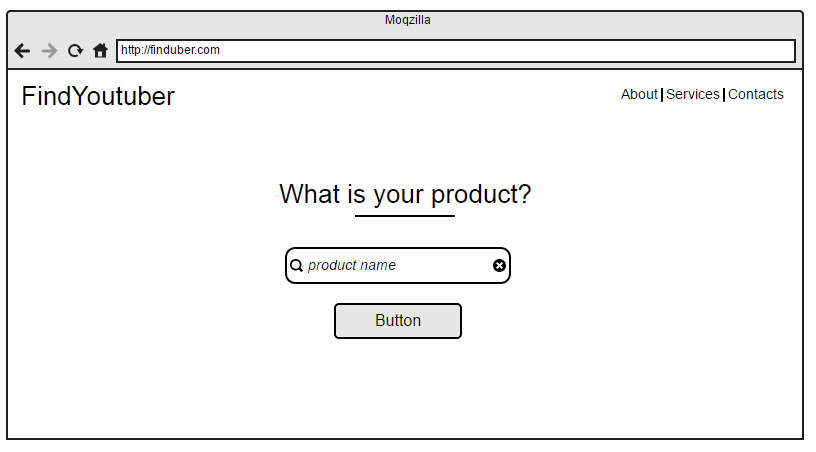
\includegraphics[width=15cm]{moch}
\caption{Page Mockup} \label{pagemockup}
\end{figure}

These three steps described represents the rough project plan. Further in the chaper are described main techniques, methods and algorithms choosen for developing the steps. It is also explained why these frameworks and technologies are more convenient for project goals. 

\subsection{Machine Learning}

Over the past two decades Machine Learning has become one of the mainstays of information technology and with that, a rather central, albeit usually hidden, part of our life. With the ever increasing amounts of data becoming available there is good reason to believe that smart data analysis will become even more pervasive as a necessary ingredient for technological progress, \cite{machinelearningdef}. 

Machine learning is a set of tools that, broadly speaking, allow us to ``teach" computers how to perform tasks by providing examples of how they should be done. For example, suppose it is need to write a program to distinguish between valid email messages and unwanted spam. For this a set of simple rules have to be written, such as flagging messages that contains certain features. However, writing rules to accurately distinguish which text is valid can actually be quite difficult to do well, resulting either in many missed spam messages, or, worse, many lost emails.

Often, machine learning methods are broken into two phases:
\begin{enumerate}
\item[--] Training: A model is learned from a collection of training data.
\item[--] Test: The model is used to make decisions about some new test data.
\end{enumerate}

Machine learning tasks are typically classified into three broad categories, depending on the nature of the learning ``signal" or ``feedback" available to a learning system. These are as specfied in \cite{machinetypes}:

\begin{itemize}

\item[--] \textbf{Supervised Learning:} in which the training data is labeled with the correct answers, e.g., ``spam" or ``ham". The two most common types of supervised learning are classification (where the outputs are discrete labels, as in spam filtering) and regression (where the outputs are real-valued).
\item[--] \textbf{Unsupervised learning:} in which it is given a collection of unlabeled data, which is need to analyze and discover patterns within. The two most important examples are dimension reduction and clustering.
\item[--] \textbf{Reinforcement learning} in which an agent (e.g., a robot or controller) seeks to learn the optimal actions to take based the outcomes of past actions.
\end{itemize}

For Finduber project first two types of categories are analysed to decide which one to use. Thus, further are analyzed classification and clustering methods.

\textbf{Classification} in machine learning is the problem of identifying to which of a set of categories (sub-populations) a new observation belongs, on the basis of a training set of data containing observations (or instances) whose category membership is known. Often, the individual observations are analyzed into a set of quantifiable properties, known variously as explanatory variables or features. An algorithm that implements classification, especially in a concrete implementation, is known as a classifier. The term ``classifier" sometimes also refers to the mathematical function, implemented by a classification algorithm, that maps input data to a category.

The basic classification task has a number of interesting variants. For example, in multi-class classification, each instance may be assigned multiple labels; in open-class classification, the set of labels is not defined in advance; and in sequence classification, a list of inputs are jointly classified. A classifier is called supervised if it is built based on training corpora containing the correct label for each input. The framework used by supervised classification is shown in Figure \ref{classification}

\begin{figure}[!ht]
\centering
\includegraphics[width=15cm]{supervised-classification}
\caption{Supervised Classification}\label{classification}, \cite{nltk}
\end{figure}

Examples of classfication problems can be: text categorization, oprical character recognition, spoken language understanding, bioinformatics and others. The most known algorithms used in classification ptoblem are Naive Bayes classifier and Kernel estimation.

The Naive Bayesian Classification represents a supervised learning method as well as a statistical method for classification. Assumes an underlying probabilistic model and it allows us to capture uncertainty about the model in a principled way by determining probabilities of the outcomes, \cite{bayesian} The main disadvantage of the algorithm is that it needs a lof of labeled data in order to have a high accuracy. Usually researches are providing sets of labeled data for some purpose, for example a set of test corpus that is used to classify a review as negative or positive. Obviously, there are no available sets of labeled data suitable for Finduber problem. That is why the Naive Bayesian classification is not the best solution in our case. 

Kernel estimation is represented by k-Nearest Neighbor algorithm, that uses the local neighborhood to obtain a prediction. The K memorized examples more similar to the one that is being classified are retrieved. Since it has a high accuracy rate (with K-nn 1 Euclidean distance the accuracy is up to 96 \%) the algorithm has many drawbacks. First, it is computationally expensive to find the k nearest neighbours when the dataset is very large. Also, the model can not be interpreted (there is no description of the learned concepts), \cite{k-neighbor}

\textbf{Clustering} is a process of partitioning a set of data (or objects) into a set of meaningful sub-classes, called clusters. The quality of a clustering result also depends on both the similarity measure used by the method and its implementation. The quality of a clustering method is also measured by its ability to discover some or all of the hidden patterns. Clustering has wide applications in

\begin{itemize}
\item[--] Economic Science (especially market research).
\item[--] Document classification
\item[--] Pattern Recognition.
\item[--] Spatial Data Analysis (create thematic maps in GIS by clustering feature spaces).
\item[--] Image Processing
\end{itemize}

Clustering algorithms are of two types, depending on problem that solve. First type is partitional, when objects are devided into non-overlapping clusters such that each data object is in exactly one subset. The hierarchical type represents a set of nested clusters organized as a hierarchy. In this case it is also used a dendrogram, that represents tree diagram frequently used to illustrate the arrangement of the clusters produced. An illustration of described types is given in Figure \ref{types}

\begin{figure}[!ht]
\centering
\includegraphics[width=15cm]{partitional}
\caption{Types of Clustering}\label{types}, \cite{typescluster}
\end{figure}

\subsection{Lexical Analysis and Text Mining} \label{ssec:lexical}

Lexical analysis is defined as process of taking an input string of characters and producing a sequence of symbols called token, that may be handled more easily by a parser. Finduber project works with database records that consists of chunks of text. In general, big chunks of text does not represent a big value. The problem is that the English spken language is vast and complex. For example, the same word might have different meanings in different circumstances. It this case the solution is to construct using text mining tools. 

Text mining is the process of extracting the useful information from the textual data. It is a research area that tries to discover knowledge from unstructured texts. Comapred to data mining tools, that are designed to handle structured data, text mining works with unstructured or semi-structured data sets such as emails, HTML files and full documents.\cite{survey} In Finduber project the unstructured data refers to raw data extracted from social media content,such as chanel description. Text mining together with lexical analysis tries to solve the issues that occur in the area of data mining, information extraction, machine learning and natural language processing. 

\subsubsection{Information Extraction}

Information extraction is the retrieval and association of information from a large number of text-based documents. The method identifies key words and relationships within the text. It does this by looking for predefined sequence in the text. This technology is very useful when dealing with large volume of text, as the Finduber project has. Also, this activity concerns processing human language texts by means of natural language processing (NLP). 

\textbf{Categorization} is another aspect of text mining and lexical analysis that is necessary for Finduber project. Categorization involves indentifying the main themes of a document by inserting the document into a pre-defined set of topics. relating the definition to the described system, the documents represents the fields from the database and the pre-defined set of topics -- the pre-defined categories. 

When categorizing a document a computer program treats the document as a 'bag of words. It only counts words that appear and, from the counts, indetifies the main topics that the document covers. In case of Finduber system categorization often relies on a databse for which categories are predefined, and relationships are identified by looking for large terms, synonyms and related terms.

To handle categorization task successfully a set of processes that work hand in hand with another form NLP kit should be implemented. Thus, the field of NLP is crucial for Finduber project.

\subsubsection{Natural Language Processing}

NLP is an area of application and research that explores how computers can be used to understand and manipulate natural language text. One of the main challenge of this field involves natural language understanging regarding human language input. Applications of NLP include a number of fields of studies, some of them are speech recognition, machine translation, artificial intelligence and natural language text processing and summarization. The last one is exactly what is need for Finduber project. In order to accomplish it a set of preprocessing methods should be done, as shown in Figure \ref{text}

\begin{figure}[!ht]
\centering
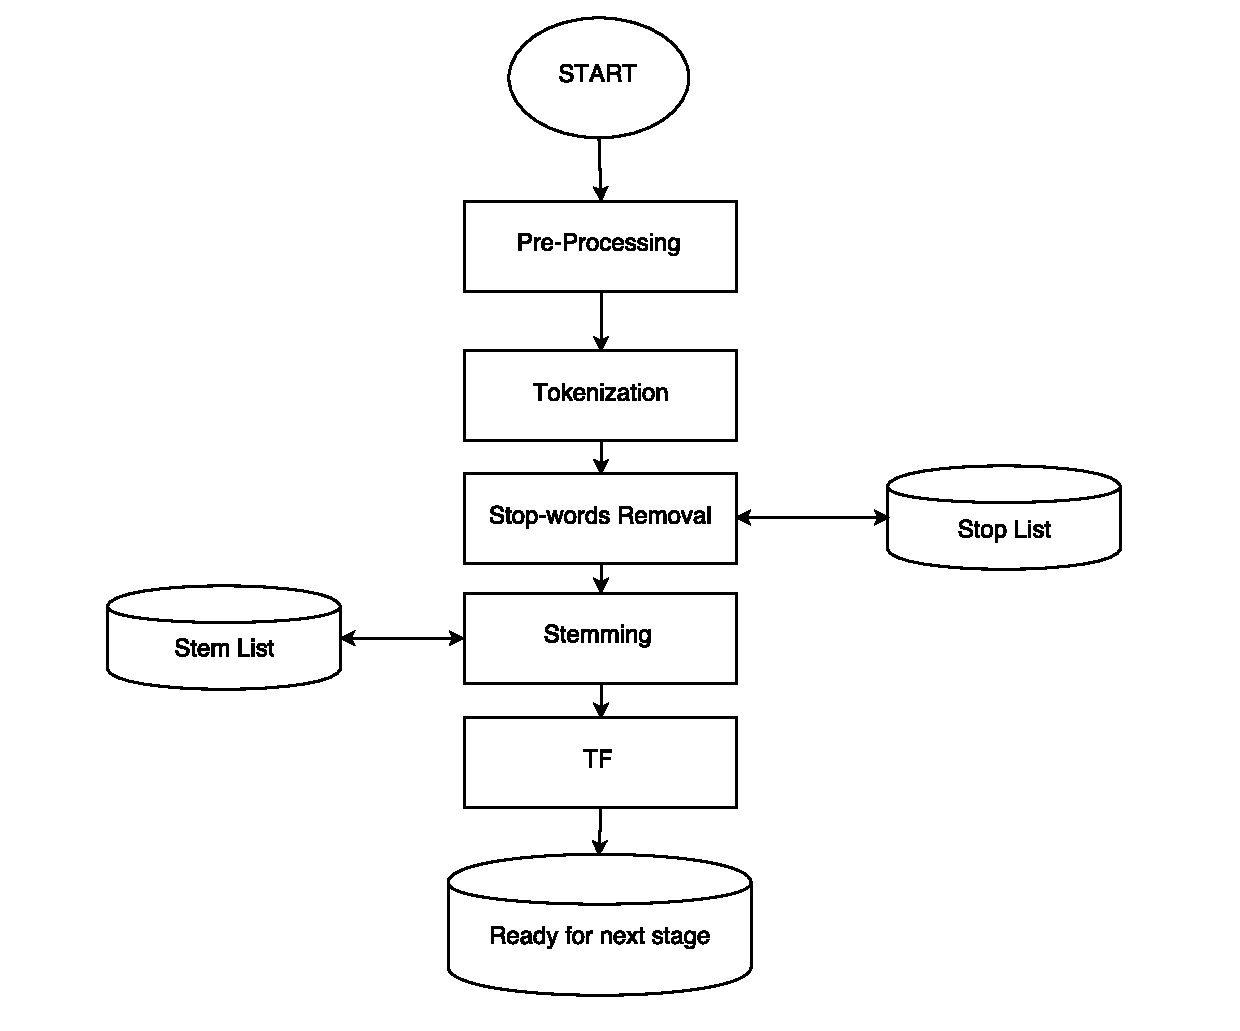
\includegraphics[width=15cm]{textmining}
\caption{Natural Language Text Processing}\label{text}
\end{figure}

\textbf{Tokenization} represents the process of breaking a string into words, phrases or other meaningful elemnts that are called tokens. The list of tokens becomes input for further processing. Tipically, segmentation occurs at the word level. Often a tokenizer relies on simple heuristics. Tokens are usually separated by white spaces. 

\textbf{Stop words eliminations} process is meant to clean the data for insigificant words. Stop words are a division of natural language. The main motive that stop-words should be removed is that they make the text look heavier and less important for analysts. The most common words in text documents are articles, pro-nouns and prepositions. Some example of stop words are: the, in, a, an, etc. Stop words are removed from documents to reduce the dimensinality of term space and because they are not treated as keywords in text mining applications. \cite{sufix}

There are three methods that can be implemented to remove stop words. 
\begin{itemize}

\item[--]{The classic method:} Is based on eliminating stop words obtained from pre-compiled lists.

\item[--]{Methods based on Zipf's Law (Z-Methods):} Additionally to the classic stop list, it uses three stop word creation methods moved by Zipf's law, including: removing most frequent words (TF-High) and removing words that occur once, i.e. singleton words (TF1). It also consider removing words with low inverse document frequency (IDF). This method is used mostly on document analysis, rather that text.

\item[--]{The Mutual Information Method (MI):} A supervised method that works by computing the mutual information between a given term and a document class (e.g., positive, negative), providing a suggestion of how much information the term can tell about a given class. Low mutual information suggests that the term has a low discrimination power and consequently it should be removed.\cite{MI}

\end{itemize}
For Finduber project the first method is more suitable, because it has to remove stop words from the text not from the documents.

\textbf{Steaming} is used to identify the root/stem of a word. For example, the words connect, connected, connecting, connections all can be stemmed to the word ``connec". \cite{stemming} The main goal of this method is to remove various suffixes, to reduce number of words and to have accurately matchin stems. There are two points that should be considered while using a stemmer:

\begin{itemize}
\item[--] Words that do not have the same meaning should be kept separate.
\item[--] The morphological forms of a word that are assumed to have the same base meaning shuld be mapped to the same stem. 
\end{itemize}

Usually, stemming algorithms can be classified into three groups: truncating, statistical and mixed methods. Each method has it way of finding the stems of the word variants. After a deep analysis of all method, the first one turns out to be the most efficient for the Finduber project. 

\textbf{Truncating Methods} are related to removing the sufixes or prefixes, i.e. affices of a word. One of the most basic stemmer is the Truncate (n) stemmer. It truncates a word at the nth symbol, thus it keeps n letter and removes the rest. Words shorter that n are kept as it is. Another approach is S-stemmer -- an algorithm conflating singular and plural forms of English nouns. It removes suffixes in plurals so as to convert them to the singular forms. \cite{truncat-stemm}

Most popular stemming algorithms used now are: Porter Stemmer and Lancaster Stemmer.

\textbf{Porter Stemmer} is one of the earliest stemming algorithms. It works by heuristically identifying word suffixes and stripping them off, with some regularization of the endings. The algorithm leaves alon strings of length one or two. 

\textbf{Lancaster Stemmer} is more aggressive than portret stemmer. With portret algorithm, the stemmed representations are usualy fairly intuitive to a reader, not so with Lancasters. However, it is faster and will reduce the set of words hugely. 

For Finduber project the Lancaster stemmer algorithm is used, because it is need to group as many words as possible according to their morphological forms.

\textbf{Term Frequency} measures how frequently a term occurs in a sequence of text.

\subsection{Wikipedia Category Tree}

Wikipedia is one of the most used and visited free-sources on the Internet. Until 2004, Wikipedia Fundation did not have a dedicted system for organizing articles. The only structure was contained in the direct links between the articles without any tools to organize them further.\cite{wikicategory} Later on in June, the Wikipedia added a feature designed to this purpose -- category pages. Through the use of category pages, it became possible to assign articles to categories and to link the these categories among themselves. Using this feature it can be created a category tree for every word that exist in wikipedia dictionary. The entire structure of organization of page hierarchy is show in the Figure \ref{category-tree-wiki}. 

\begin{figure}[!ht]
\centering
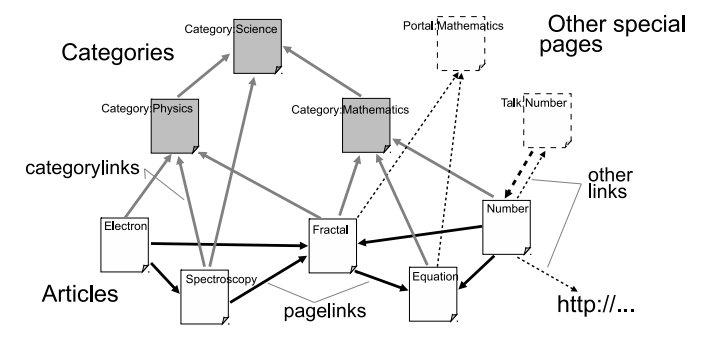
\includegraphics[width=15cm]{categorytreewiki}
\caption{Illustration of Wikipedia’s Organization of Different Pages}\label{category-tree-wiki}, \cite{wikicategory}.
\end{figure}

These structure is quite complex, but it is the suitable approach to be implemented in order to create taxonomy databases. For Finduber project only categories will be extracte, without articles and other special pages. These additional vertices are subject for future improvement of the project. To be able to extract these information from the wikipedia web page, wikipedia API is used.

\textbf{Wikipedia API} is a strong web service, that allows developers to access, search and integrate Wikipedia content into custom web applications or for information storage. This API, that works over HTTP and returns data in a variety of different formats, including XML, is freely available to the programming public and makes it possible to create all kinds of custom web applications powered by Wikipedia's huge content database. Details about how it is implemented and how to fetch data from it are described in Chapter 3.

\subsection{Big Data}

Finduber project deals with biga data analysis and storage. Because the data from the database with youtube users represents an unstructured data and it size is over four gigabytes. In these subsection is defined the term of big data and how it is relate to social media, are analyses technologies used for big data analysis and efficient methods of data storage. 

Every day people around the world post 400 million tweets on Twitter, add 350 million photos to Facebook and view 4 billion videos on YouTube.\cite{digitalInfo} Every 60 seconds on Facebook are posted 510 comments and 293,000 statuses are updated.\cite{zephoria} This has prompted the development of new technical and methodological approache to capture, process and analyse large and complex data, called \textbf{Big Data}. 

A 2011 paper by the McKinsey Global Institute describes big data thus: ``Big data refers to datasets whose size is beyond the ability of typical database software tools to capture, store, manage, and analyze."\cite{bigdata} 

Big data aprroaches to analysing social media data can increase undertanding of how people think and act. Companies can use the information obtained to improve decision-marking, target services and products more effectively and to try to influence users' decisions and behaviours in the future.\cite{POSTNOTE460}

The rate of unstructured data production on social media makes it difficult to analyse and store it using traditional methods. Traditional methods of management system and analytics systems are based on the relational database management system (RDBMS) and can only be applied to structured data.\cite{bdtech} Due to this problem, research community has proposed some solutions that could storage and analyse big data, these solutions and technologies are described in the next subsections.

\subsubsection{Hadoop and MapReduce}

One of the fundamental technologies related to big data is \textbf{Hadoop}, that forms a powerful big data systematic solution through data storage, data processing, runing applications on clusters and integration of other modules. 

It was initially developed by Doug Cutting and Mike Cafarella as an open-source web search ingine called Nutch. Its purpose was to return web search results faster by distributing data and calculations across different computers so multiple tasks could be acccomplished simultaneously. Later the project was devided - the web crawler part remained as Nutch and the distributed computing and processig part became Hadoop.\cite{sas} Today Hadoop is managed and maintained by the Apache Software Foundation (ASF) and is widely used by big Internet enterprises like Facebook, Yahoo. 

Hadoop consists of two parts: HDFS (Hadoop Distributed File System) and MR framework (MapReduce Framework). HDFS stores data from different external sources fed into a Hadoop cluster. A HDFS cluster includes a single NameNode for managing the metadata of the file system and DataNodes for storing actual data.The MR framework consist of one JobTraker and and multiple TaskTraker nodes.

The described architecture of Hadoop is shown in the \mbox{Figure \ref{hdfs_arch}}.

\begin{figure}[!ht]
\centering
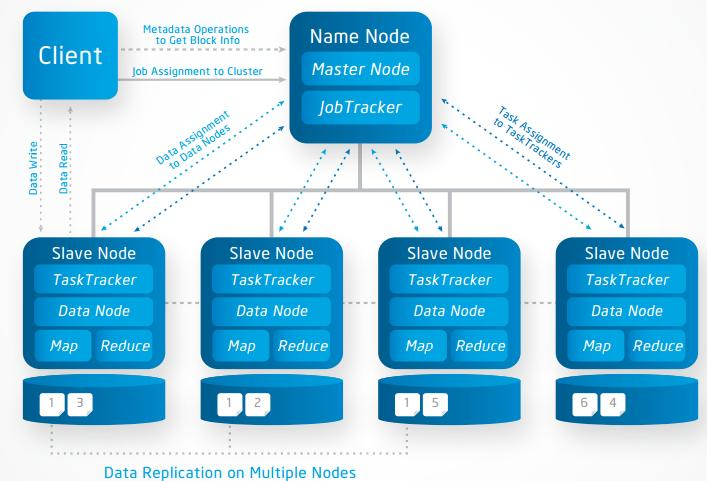
\includegraphics[width=15cm]{hdfs_architecture}
\caption{Hadoop Architecture\cite{hdfsFigure}}\label{hdfs_arch}
\end{figure}

During injection, the data is broken down into smaller chunks. The master node holds all the metadata information regarding the data split up and this enables it to recreate the whole data set using different slave machines.\cite{blog} The client submits a Job to the master node and it in turn assigns the Job to the slave nodes. For assigning the tasks to the salve nodes is respnsible the Jobtracker process that runs on the master node. The task is not run on all the data that is hold on the salve node but only on the data slice that has been specified by the Master Node. The slaves run TaskTracker, HDFS to store data, and map and reduce functions for data computation.\cite{rosebt} If one of the data replicas on HDFS is corrupdet, JobTracker, will look for an alternate slave node that contains the same data. 

MR in complement to a RDBMS is a good fit for problems that need to analyze the whole dataset in a batch fashion and unstructured data. Because, in the case of MR framework, data is partitioned the functional primitives (map and reduce) cand work in parallel on separate partitions. More differences between MR and RDBSMS are shown in \mbox {Table \ref{table:mrdiff}}:

\begin{table}[!ht]
\begin{center}
\caption{RDBMS compared to MapReduce \cite{tableHadoop}}
\begin{tabular}{| c | c | c |}
\hline
  & \textbf{Traditional RDBMS} & \textbf{MapReduce} \\
\hline
 \textbf{Data size}& Gigabytes & Petabytes \\
\hline
 \textbf{Access}& Interactive and batch & Batch \\
\hline
\textbf{Updates} & Read and write many times & Write once, read many times \\
\hline
\textbf{Transactions} & ACID & None \\
\hline
\textbf{Structure} & Schema-on-write & Schema-on-read \\
\hline
\textbf{Integrity} & High & Low \\
\hline
\textbf{Scaling} & Nonlinear & Linear \\
\hline
\end{tabular}
\label{table:mrdiff}
\vspace{-2.5em}
\end{center}
\end{table}

The main advantages of Hadoop are:
\begin{itemize}

 \item \textit{High Cost Efficiency} - since large-sclae parallel computing to commercial servers is applied, the cost per terabyte required for storage capacityis greatly reduced.

 \item \textit{Strong Flexibility} - handle many kinds of data from various sources.

 \item \textit{Expandability} - expansion or shrinkage of hardware infrastructure without changing data format.

 \item \textit{High Fault-Tolerance} - recover data and correct computing errors caused by node failures.

\end{itemize}

Having the Hadoop technology that allows to store and analyse big data, the main questions are: Which is the best way of storing the data? What methods are used for data anlysis? 

\subsubsection{Big Data Storage}

Data storage is related to the storage and managemet of large-sclae datasets, while achieving reliability and availability. Storage systems shall be equipped with many interfaces, rapid query, or other type of programming models for analysing of stored data and interaction with it. Traditionally, data storage equipment manages, looks up and analyzes data with structured RDBMSs. But since the volume of the big data is measured in terabytes and petabytes makes traditional storage equipment and management modes inadequate. Therefore, there is a compelling need for research on data storage.\cite{bdtech}

In order develop a large scale distributed storage system for  efficient data processing and analysis the following factors should be taken in consideration:\cite{CAP}

\begin{itemize}

\item \textit{Consistency} - all nodes see the same data at the same time.
\item \textit{Availability} - a guarantee that every request receives a response about whether it succeeded or failed.
\item \textit{Partition tolerance} - the system continues to operate despite arbitrary partitioning due to network failures.

\end{itemize}

In 2000 Eric Brewer proposed a CAP theory, that stated that in a distributed system could not have all this three factors enumerated above simultaneously. The theory was proved two years later by Seth Gibert and Nancy Lynch from MIT. According to the theory we can have a CA system, where partition tolerance is sacrificed, a CP system by ignoring availability and an AP system where consistency element is missing.

\textbf{CA} systems could not handle network failures, because the partition tolerance is missing, this is why they are storage systems with a single server and could not be expanded. So, for large-scale stored systems are used CP systems and AP systems. 

\textbf{CP} systems ensure partition tolerance, in such a way the system can be expanded to become a distributed one. To ensure a level of partition tolerance system maintain several copies of the same data. The copies are completely identical, thus ensuring cosistency. Because CP systems do not have the third factor, availability, to guarantee a response to every request, system will wait for a response from the partitioned node that could reuslt in a timeout error. CP systems are chosen when the amount of data is not so big. Examples of CP systems are: BigTable and Hbase.

\textbf{AP} systems ensure availability and partition tolerance. The consistency factor is missing, therefore AP systems are applied to the scenarios with frequent req
uests but not very high requirements on accurancy. Availability is also an option when the system needs to continue to function in spite of external errors\cite{AP} for example in online Social Network Services. Two popular AP systems are Dynamo and Cassandra. 

\textbf{Database Technology} is also used to store data. Every complex system requires a database technology to handle datasets at different scales. It is apparent that traditional relational databases cannot meet the challenges on categories and scales brought about by big data. In this context NoSQL databases are becoming more used and popular for big data storage. Compared with relational databases, NoSQL ones feature flexible models, simple API, eventual consistency and support of large volume data. There are three main NoSQL databases:
 
\begin{itemize}
\item[--] Key-value databases.
\item[--] Column-oriented databases.
\item[--] Document-oriented databases.
\end{itemize} 

\textbf{Key-value databases} store data corresponding to key-values. Every key is unique and customers may input queried values according to the keys. Such structure is simple and is characterized with high expandability. You can find the value data based on searching the key field, in this way the query time is much smaller than for relational databases.

Key-value stores are used in massive multi-player on-line gaming to manage each player session, in managing the shopping cart transactions up to the point of payment. Example of such database are: Redis, Memcached, Voldemort, Amazon Dynamo DB.

\textbf{Column-oriented databases} store data tables according to columns rather that rows. To realize expandability columns and rows are segmented in multiple nodes. The column-oriented databases are mainly inspired by Google's BigTable. Cassandra is another example of database from this category.

\textbf{Document-oriented databases} can support more complex data forms, compared with key-values database. Moreover, is no need to conduct mode migrations, because documents do not follow strict models. The application logic is much easier to write for document-oriented databases, since it is not need to translate between objects in application and SQL queries, object model can just be turned directly into a document.

Document databases have very powerful query engines and indexing features that make it easy and fast to execute many different optimized queries. \cite{mongodb-adv} Three important representatives of document stoarge systems are: MongoDB, SimpleDB and Couch DB. 

As was mentioned at the beginning of the chapter, the Finduber project uses two databases. The youtube database uses PostgreSQL to store the data. For taxonomy database it is choosen the document-based model -- MongoDB. This model is the most optimal choise, because it supports documents hierarchy and this is exactly what is need for storing a category tree.

\subsection{PostgreSQL Indexing in Rails}

Postgres, is an object-relational database management system (ORDBMS) with an emphasis on extensibility and standards-compliance. Although is not a NoSQL database, it has a long track record of use in data warehouse. For a decade before Hadoop launched, PostgreSQL was the only pure open-source option for large data volumes and complex analytics. One thing relational database do a lot of is sorting data. The bigger the database size, the more the performance of those sorts becomes the dominating factor in overall response time.\cite{whypostgres} To solve this problem, newer versions of PostgreSQL supports indexing. 

Indexes are a common way to enhance database performance. An index allows the database server to find and retreive specific rows much faster. But they also add overhead to the database system as a whole, so they should be used sensibly.

PostgreSQL includes four index types: B-tree, Hash, GiST and GIN, each of them using a different algorithm that is best suited to different types of queries. B-tree index type is the most commonly used index type for most use cases, that is way it will be used in Finduber project as well. The main drawback of hash indexes is that they cannot be recovered after a crash of power loss. 

B-tree is a self-balancing tree data structure that keeps data sorteed and allows searches, insertions, deletions and sequential access in logarithmic time. In particular, the PostgreSQL query planner will consider using a B-tree index whenever an indexed column is involved in a comparison using one of these operators: \textless, <=, =, >= and \textgreater. Constructs equivalent to combinations of these operators, such as BETWEEN and IN, can also be implemented with a B-tree index search. Also, an IS NULL or IS NOT NULL condition on an index column can be used with a B-tree index.\cite{postgresweb} Using B-tree indexes can be created primary keys, foreign keys, uniques indexes and sorted indexes. 

In general it's a good practice to add an index for primary key in database tables. Since the number of youtube users is huge, the database tables will have a large number of rows. That is why it is need of an index, thus the lookup will take place in the index instead of sequentially scan the tables for the matching rows. Luckily, PostgreSQL automatically creates an index for primary keys to enforce uniqueness. Thus, it is not necessary to create an index explicitly for primary key columns. An example is shown in listing \ref{primarykey}. 

\lstinputlisting [language=Ruby, caption={Primary Key Index in Rails}, label=primarykey]{../src/primary_key.rb}

\newpage

This creates a primary key index using the B-tree type to index the id column. In postgres table description it will look like: 

\lstinputlisting [language=SQL, caption={Primary Key Index in PostgreSQL Console}, label=primarykey]{../src/psql.sql}

Compared to primary keys, foreign keys of the table are not indexed automatically in Rails. Their purpose is to make association between multiple tables. If the developer wants to link two tables from the database using foreign key, it should define it in the database schema. For example notation shown in listing \ref{indexes} will associate table products with table categories, that has a row called category\_id.

Another important type of index, that is used in Finduber project is sorted index. It comes to help to handle SELECT queries with WHERE clause used over a big number of rows. Tom Ward in his blog post ``Using indexes in rails: Index your associations" made an experiment to test the efficiency of using sorted indexes. He took a sql query and ran it on a database with 1 million rows. Then Tom Ward added a sorted index to the database and run the same query on the same database. The result of the experiment is shown in Table \ref{table:sql_results}

\begin{table}[!ht]
\begin{center}
\caption{Execution Time of SQL Queries \cite{experiment_results}}
\renewcommand{\arraystretch}{2}
\begin{tabular}{| c | >{\centering\arraybackslash}p{7.5cm}  | >{\centering\arraybackslash}p{5cm} | c |}
\hline
\textbf{Key}& \textbf{SQL query} & \textbf{Execution Time} & \textbf{Rows} \\
\hline
\textbf{NULL} & \pbox{20cm}{SELECT * FROM conversations \\ WHERE user\_id = 41;} & 1.42 sec & 1001111 \\
\hline
\textbf{used\_id\_ix} & \pbox{20cm}{SELECT * FROM conversations \\ WHERE user\_id = 41;} & 0.01 sec & 108 \\
\hline
\end{tabular}
\label{table:sql_results}
\vspace{-2.5em}
\end{center}
\end{table}

\vspace{10 pt}

Key column shows the index that database decided to use, in first case it is NULL as there were no indexes, but in the second case it uses the added index -- user\_id\_ix careted as in listing \ref{indexes}. The rows column is also relevant, it shows at how many rows the database will need to look to give the results. 
The difference is remarkable. Using sorted index the query was executed only in 0.01 seconds that means an increase of 99.3 \%. It is due the fact that the query do not look in the all database, but only through  108 rows. The experiment demonstrates that the usage of sorted indexes totally worth it. 

It is also possible to add aditional clauses to the sorted index. For Finduber project ORDER BY clause is needed. By default, the entries in a B-tree index is sorte in ascending order, but for the system the descending order is required. In listing \ref{indexes} is shown an example of sorted index creation that group articles from the tabel posts, sorted in descending order by released\_at column. For unreleased articles, the released\_at value is NULL.

Unique indexes for a column are used to guarantee that the table won't have more than one row with the same value for that column. This types of indexes are mainly used in the systems where users can create accounts. In this case using only validation in the model isn't enough to enforce uniquencess. Because if two users will hit the ``Sign up" button at the same time, Rails will search in the user table for that credentials and respond back there is no such record and it can be saved in the table. Thus, two records with the same email address, for example, will be saved in the database. To avoid this and ensure that table users will have uniques records in email field is need to create an unique index as specified in listing \ref{indexes}

\lstinputlisting [language=Ruby, caption={Creation of Foreign, Unique and Sorted Keys in Rails}, label=indexes]{../src/foreign.rb} 















